\documentclass{article}
\bibliographystyle{alpha}
\usepackage[utf8]{inputenc}
\usepackage{makeidx}  \usepackage{graphicx}
\usepackage{balance}
\usepackage{listings}
\usepackage{multirow}
\usepackage{threeparttable}
\usepackage{booktabs}
\usepackage{epstopdf}
\usepackage{amsmath,amsfonts,amssymb,mathrsfs,amsthm}
\usepackage{float}                              \usepackage{multirow}
\usepackage{caption}
\usepackage{subfig}
\usepackage{footnote}
\usepackage{color}
\usepackage{pifont}
\usepackage{acronym}
\usepackage{lscape}

\usepackage{pgfplots}
\pgfplotsset{compat=newest}
\usetikzlibrary{plotmarks}


\newlength\figureheight
\newlength\figurewidth
\setlength\figureheight{5cm}
\setlength\figurewidth{6cm}




\definecolor{rosso}{RGB}{220,57,18}
\definecolor{giallo}{RGB}{255,153,0}
\definecolor{blu}{RGB}{102,140,217}
\definecolor{verde}{RGB}{16,150,24}
\definecolor{viola}{RGB}{153,0,153}

\makeatletter

\tikzstyle{chart}=[
    legend label/.style={font={\scriptsize},anchor=west,align=left},
    legend box/.style={rectangle, draw, minimum size=5pt},
    axis/.style={black,semithick,->},
    axis label/.style={anchor=east,font={\tiny}},
]

\tikzstyle{bar chart}=[
    chart,
    bar width/.code={
        \pgfmathparse{##1/2}
        \global\let\bar@w\pgfmathresult
    },
    bar/.style={very thick, draw=white},
    bar label/.style={font={\bf\small},anchor=north},
    bar value/.style={font={\footnotesize}},
    bar width=.75,
]

\tikzstyle{pie chart}=[
    chart,
    slice/.style={line cap=round, line join=round, very thick,draw=white},
    pie title/.style={font={\bf}},
    slice type/.style 2 args={
        ##1/.style={fill=##2},
        values of ##1/.style={}
    }
]

\pgfdeclarelayer{background}
\pgfdeclarelayer{foreground}
\pgfsetlayers{background,main,foreground}


\newcommand{\pie}[3][]{
    \begin{scope}[#1]
    \pgfmathsetmacro{\curA}{90}
    \pgfmathsetmacro{\r}{1}
    \def\c{(0,0)}
    \node[pie title] at (90:1.3) {#2};
    \foreach \v/\s in{#3}{
        \pgfmathsetmacro{\deltaA}{\v/100*360}
        \pgfmathsetmacro{\nextA}{\curA + \deltaA}
        \pgfmathsetmacro{\midA}{(\curA+\nextA)/2}

        \path[slice,\s] \c
            -- +(\curA:\r)
            arc (\curA:\nextA:\r)
            -- cycle;
        \pgfmathsetmacro{\d}{max((\deltaA * -(.5/50) + 1) , .5)}

        \begin{pgfonlayer}{foreground}
        \path \c -- node[pos=\d,pie values,values of \s]{} +(\midA:\r);
        \end{pgfonlayer}

        \global\let\curA\nextA
    }
    \end{scope}
}

\newcommand{\legend}[2][]{
    \begin{scope}[#1]
    \path
        \foreach \n/\s in {#2}
            {
                  ++(0,-10pt) node[\s,legend box] {} +(5pt,0) node[legend label] {\n}
            }
    ;
    \end{scope}
}



\acrodef{PV}{photovoltaic}
\acrodef{HEMS}{home energy management system}
\acrodef{NILM}{non-intrusive load monitoring}
\acrodef{HMM}{Hidden Markov Model}
\acrodef{FHMM}{Fractional Hidden Markov Model}
\acrodef{HSMM}{Hidden Semi-Markov Models}
\acrodef{PF}{particle filtering}
\acrodef{ILM}{intrusive load monitoring}
\acrodef{FSM}{Finite State Machine}
\acrodef{RMSE}{root mean square error}
\acrodef{ACC}{Accuracy}
\acrodef{SPARQL}{SPARQL Protocol and RDF Query Language}
\acrodef{RDF}{Resource Description Framework}
\acrodef{SPIN}{SPARQL Inferencing Notation}
\acrodef{BLH}{battery load hiding}
\acrodef{LLH}{load based load hiding}
\acrodef{OWL}{ontology web language}

\definecolor{orange}{rgb}{1,0.5,0}

\newcommand{\cmark}{\ding{51}}\newcommand{\xmark}{\ding{55}}


\begin{document}






\title{Integration of Legacy Appliances into Home Energy Management Systems}



 \author{
Dominik~Egarter, Andrea~Monacchi, Tamer~Khatib, \\
and~Wilfried~Elmenreich\
ACC = \frac{TP+TN}{N} \in [0,1],

{RMSE} = \frac{\sqrt{E((\hat{\Theta}-\Theta))^2}}{max(\Theta)-min(\Theta)},

where  represents the true total power load,  the estimated total power load produced by \ac{PF} and  and  the maximum and minimum power value of the total power load.
  \item \textit{Energy disaggregation error} The percentage error of the estimated energy with respect to the real consumed energy, over the duration of the experiment.
\end{itemize}

\subsubsection{Results}


As described before, we considered different test scenarios for our evaluations.
The first one deals with the aggregated power demand of seven appliances listed in Table \ref{tab:applianceList}.
In Table \ref{tab:aggregatedResults} the evaluation results are presented.
The reached \ac{ACC}, \ac{RMSE} and disaggregation error depend on the complexity of devices (e.g.: on/off or multi-state appliances) and the similarity of devices regarding their power demand.
For example, the set of TV, fridge and washing machine yields a decreased \ac{ACC} and \ac{RMSE} due to their appliance type and their similarity of consuming power.

\begin{figure}
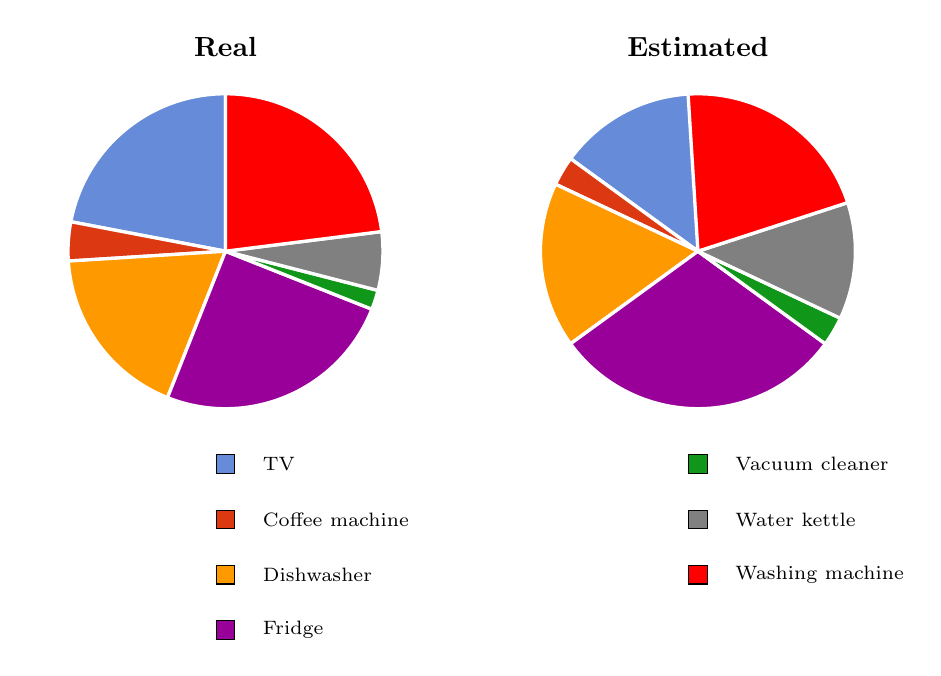
\begin{tikzpicture}
[
    pie chart,
    slice type={TV}{blu},
    slice type={coffee}{rosso},
    slice type={dishwasher}{giallo},
    slice type={fridge}{viola},
    slice type={vaccuum}{verde},
    slice type={waterkettle}{gray},
    slice type={washingmachine}{red},
    pie values/.style={font={\small}},
    scale=2
]

    \pie[values of coffee/.style={pos=1.2},values of vaccuum/.style={pos=1.2}]
    {Real}{22/TV,4/coffee,18/dishwasher,25/fridge,2/vaccuum,6/waterkettle,23/washingmachine}
    \pie[xshift=3cm,values of coffee/.style={pos=1.2},values of vaccuum/.style={pos=1.2}]{Estimated}{15/TV,3/coffee,17/dishwasher,30/fridge,3/vaccuum,12/waterkettle,21/washingmachine}

    \legend[shift={(0cm,-1cm)}]{{TV}/TV, {Coffee machine}/coffee, {Dishwasher}/dishwasher,{Fridge}/fridge}
    \legend[shift={(3cm,-1cm)}]{{Vacuum cleaner}/vaccuum,{Water kettle}/waterkettle,{Washing machine}/washingmachine}

\end{tikzpicture}
\caption{Sketch of the household energy partition on appliance level for the measured and estimated case are shown}
\label{fig:aggregatedEnergy}
\end{figure}
In Figure \ref{fig:aggregatedEnergy} the energy partition on the real and the estimated energy computation on appliance level is shown. 
The estimated energy values and their corresponding percentages on the overall energy demand show again the dependence of the load disaggregator on the appliance type and the similarity between appliances.

\begin{figure}
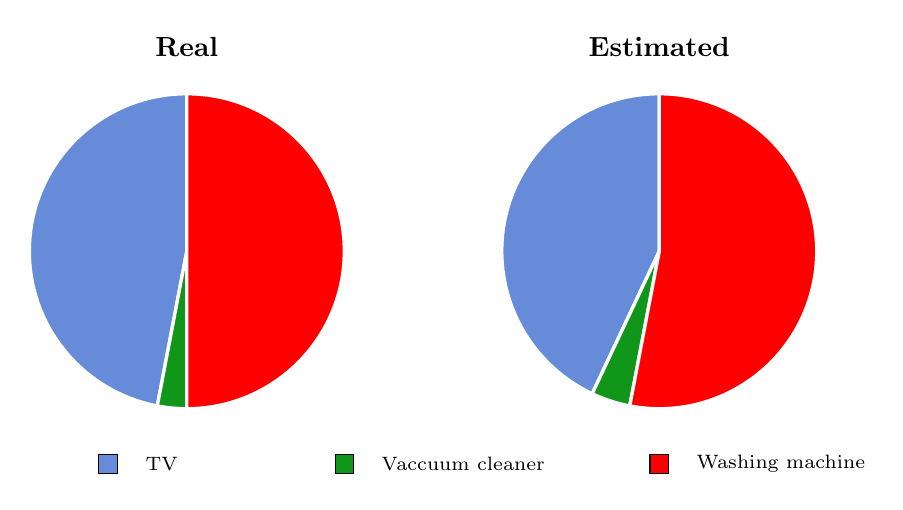
\begin{tikzpicture}
[
    pie chart,
    slice type={TV}{blu},
    slice type={vaccuum}{verde},
    slice type={washingmachine}{red},
    pie values/.style={font={\small}},
    scale=2
]

    \pie[values of vaccuum/.style={pos=1.2}]
    {Real}{47/TV,3/vaccuum,50/washingmachine}
    \pie[xshift=3cm,values of coffee/.style={pos=1.2},values of vaccuum/.style={pos=1.2}]{Estimated}{43/TV,4/vaccuum,53/washingmachine}

    \legend[shift={(-0.5cm,-1cm)}]{{TV}/TV}
    \legend[shift={(1cm,-1cm)}]{ {Vaccuum cleaner}/vaccuum}
    \legend[shift={(3cm,-1cm)}]{{Washing machine}/washingmachine}
\end{tikzpicture}
\caption{Sketch of the household energy partition on appliance level for the measured and estimated case are shown in which appliances are formed into group 0 (TV, vacuum cleaner, washing machine)}
\label{fig:grouped_1_aggregatedEnergy}
\end{figure}

\begin{figure}
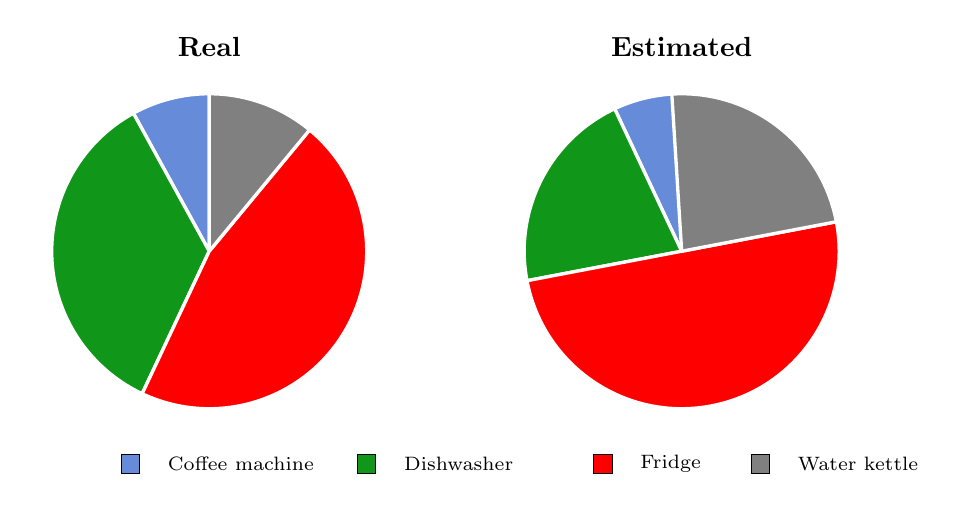
\begin{tikzpicture}
[
    pie chart,
    slice type={coffee}{blu},
    slice type={dishwasher}{verde},
    slice type={fridge}{red},
    slice type={waterkettle}{gray},
    pie values/.style={font={\small}},
    scale=2
]

    \pie
    {Real}{8/coffee,35/dishwasher,46/fridge,11/waterkettle}
    \pie[xshift=3cm]{Estimated}{7/coffee,21/dishwasher,50/fridge,23/waterkettle}

    \legend[shift={(-0.5cm,-1cm)}]{{Coffee machine}/coffee}
    \legend[shift={(1cm,-1cm)}]{ {Dishwasher}/dishwasher}
    \legend[shift={(2.5cm,-1cm)}]{{Fridge}/fridge}
      \legend[shift={(3.5cm,-1cm)}]{{Water kettle}/waterkettle}
\end{tikzpicture}
\caption{A Sketch of the household energy partition on appliance level for the measured and estimated case are shown in which appliances are formed into group 1 (coffee machine, dishwasher, fridge, water kettle)}
\label{fig:grouped_2_aggregatedEnergy}
\end{figure}
In the second test scenario appliances are grouped to decrease the number of appliances.
The results of \ac{ACC} and \ac{RMSE} are shown in Table \ref{tab:groupedResults} and are improved compared to Table \ref{tab:aggregatedResults}.
As reason we assume the decreased number of appliances and the corresponding decreased probability to have similar appliances in the same appliance group.
Figure \ref{fig:grouped_1_aggregatedEnergy} and \ref{fig:grouped_2_aggregatedEnergy} show the energy partitions of the submetered demand for the real and the estimated energy values.
As in the previous test scenario, similar appliances influence the result of the disaggregator.
In summary, a load disaggregator could be used to disaggregate appliances from the aggregated household power demand.
The performance is mainly affected by the number of considered appliances, the type of appliances and their similarity.
Note that the presented load disaggregator is aware of the appliance type/model and the number of appliances.
Although it is one of numerous \ac{NILM} approaches applicable for this problem, the presented approach appears to be a good choice fulfilling the requirements given by Zeifman.
Nevertheless, to achieve full integration of legacy devices in a \ac{HEMS}, a load disaggregator has to combine appliance detection with signature extraction approaches.
While appliance detection provides information of appliance status and allows for the inference of device profiles (see Sect. \ref{subsec:nilmrepresentation}),
signature extraction allows for the inference of device models, to be used for improving the appliance detection process.

\begin{table}
 \centering
 \begin{tabular}{|c|cc|}
\hline
&  \ac{ACC} & \ac{RMSE} \\
\hline
\hline
TV 							& 0.8705	& 0.2995 \\
Coffee machine 				& 0.9901	& 0.0673 	 \\
Dishwasher 					& 0.9549	& 0.1263 \\
Fridge						& 0.8992	& 0.2095 \\
Hoover						& 0.9952	& 0.0649 \\
Water kettle  				& 0.9827	& 0.1131\\
Washing machine				& 0.8826	& 0.1251\\
\hline
\hline
Total						& 0.9393	& 0.051 \\
\hline
\end{tabular}
\caption{Results for test scenario 1}
\label{tab:aggregatedResults}
\end{table}


\begin{table}
 \centering
 \begin{tabular}{|c|cc|}
\hline

&  \ac{ACC} & \ac{RMSE}  \\
\hline
\hline
& \multicolumn{2}{c|}{Group 1} \\
\hline
Coffee machine 			& 0.994		& 0.0332   \\
Dishwasher 				& 0.9626	& 0.0941  \\
Fridge 					& 0.994 	& 0,0742 \\
Water kettle			& 0.9889	& 0.0948 \\
\hline
Total 					& 0.9849	& 0.0091  \\
\hline
\hline
& \multicolumn{2}{c|}{Group 2} \\
\hline
Vacuum cleaner			& 0.9643	& 0.1548  \\
Washing machine  		& 0.997		& 0.152	\\
TV 						& 0.9456	& 0.0186  \\
\hline
\hline
Total 					& 0.9699 & 0.0101  \\
\hline
\end{tabular}
\caption{Results for test scenario 2}
\label{tab:groupedResults}
\end{table}

\subsection{Annotation of inferred information}
In order to model device profiles and device models, we used the the open source tool Prot\'eg\'e\footnote{http://protege.stanford.edu} to build models in the \ac{OWL}.
The resulting ontology is available for use at the MONERGY project webpage\footnote{http://www.monergy-project.eu/appliance-ontology/}.
Fig.~\ref{fig:datasheetkettle} shows an example profile for a water kettle.
The device is user driven and has a physical service to heat water.
The service demands 0.03 KWh and is currently in the OFF status.
The service takes place over one state, requiring 1800 W with 5\% tolerance being insensitive to interruption and start delay.
\begin{figure}[h!]
\centering
\includegraphics[width=\columnwidth]{figure6}
\caption{Device profile for the water kettle}
\label{fig:datasheetkettle}
\end{figure}
Fig.~\ref{fig:nilmmodelkettle} reports the load identification model for the water kettle.
To identify the device, this model describes OFF and ON observations, using active power as a feature.
As noticeable, device dynamics are captured using transition probabilities.
\begin{figure}[h!]
\centering
\includegraphics[width=\columnwidth]{figure7}
\caption{Load identification model for the water kettle}
\label{fig:nilmmodelkettle}
\end{figure}

\section{Conclusions}\label{sec:conclusion}
This paper addressed the problem of device and data interoperability in HEMS.
In particular we analyzed building blocks of a \ac{HEMS} to identify main challenges.
We put ahead a general architecture for \ac{HEMS}, where requirements and characteristics are presented.
Although the current standardization effort will soon provide technologies to design smart appliances, many energy consuming and producing devices will be non-smart. Replacing all legacy devices by smart devices would be economically infeasible in many situations. Therefore, such legacy devices are assumed to have a significant impact on the energy consumption and thus, deserve consideration within energy management applications.
We discussed the application of load detection for the identification of running loads, as well as the integration of inferred information into HEM systems.
We advocate for a common description for smart and legacy devices, as it would offer a uniform interface to access features and data, with consequent complexity reduction for application developers.
A case study is provided to show the effectiveness of a load disaggregation algorithm on real data collected from a living environment.
We carried out two different approaches to monitoring and disaggregating appliances where the load disaggregator inputs the aggregated power profile of i) all appliances and ii) grouped devices.
A state-of-the-art load detection algorithm was applied to identify which monitoring approach is suitable to integrate legacy appliances into a \ac{HEMS}.
Our results demonstrate that each monitoring approach allows for the correct detection and therefore integration of appliances, according to the requirements defined.
We pointed out different advantages and disadvantages of these approaches, which should be considered during the design of the \ac{HEMS}.
We also showed how similarities between electrical devices affect the disaggregation process negatively.
Finally, we exercise how information from detected appliances can be annotated to be exchanged within a \ac{HEMS}.
To the best of our knowledge, this is the first paper showing how the integration of legacy devices into the \ac{HEMS} could take place, what requirements should be fulfilled and which limitations and challenges need to be considered.

\section{Acknowledgments}
This work was supported by Lakeside Labs GmbH, Klagenfurt, Austria and funding from the European Regional Development Fund and the Carinthian Economic Promotion Fund (KWF) under grant KWF-. 



\bibliography{dominik,andrea}

\end{document}
